\documentclass[a4j, 10pt, twocolumn]{ltjarticle}  % 「ltjsarticle」は見た目変わるので注意
\usepackage{graphicx}
\usepackage{float}
\usepackage{wrapfig}
\usepackage{amsmath, amssymb, amsfonts}
\usepackage{latexsym}
\usepackage{color}
\usepackage[normalem]{ulem}
\usepackage[hyphens]{url}
\usepackage{bm}
\usepackage{here}
\usepackage{multirow}
\usepackage{lltjext}

% ==============================================
% ページ設定のレイアウト確認
% \usepackage{layout}
% 本文中で「\layout」を呼び出す
% ==============================================
% ページ設定
% documentclass「a4j (210*297mm)」を基準とする
% 1inch = 72pt = 25.2mm
% 1pt = 0.35mm
\usepackage{geometry}
\geometry{
    top=21mm,  % 上部の余白領域
    bottom=21mm,  % 下部の余白領域
    inner=21mm,  % 左部の余白領域
    outer=21mm,  % 右部の余白領域
    headheight=0mm,  % ヘッダーの領域
    headsep=0mm,  % ヘッダーと本文領域の間隔('headheight'と'headsep'を0にするなら'nohead'でも良い)
    % nohead,
    columnsep=10mm,  % 2段組の中央の間隔
    marginparwidth=0mm,  % Margin Notesの領域
}
\pagestyle{empty}
% ==============================================
% コマンドのカスタマイズ
\makeatletter
\renewcommand{\section}{\@startsection{section}{1}{\z@}
   {1.5\Cvs \@plus.5\Cvs \@minus.2\Cvs}
   {.5\Cvs \@plus.3\Cvs}
   {\reset@font\large\bfseries}}  % section見出しの文字サイズをlargeに変更
\renewcommand{\subsection}{\@startsection{subsection}{2}{\z@}
   {1.5\Cvs \@plus.5\Cvs \@minus.2\Cvs}
   {.5\Cvs \@plus.3\Cvs}
   {\reset@font\normalsize\bfseries}}  % subsectoin見出しの文字サイズをnormalsizeに変更
\makeatother
% ==============================================
% 本文 
\begin{document}
    % \layout
    \renewcommand{\thepage}{\arabic{page}}
    \setcounter{page}{1}
    \twocolumn[
        \vspace*{-30pt}  % 位置調整
        % 発表番号
\begin{flushright}
    \textbf{\large A1-2}
\end{flushright}
% タイトル
\begin{center}
    \textbf{\large {A1-2 CtoCシェアサイクルサービスにおける新しいマッチングモデルの提案と実装}}
\end{center}
\begin{center}
工学研究科 知識社会基礎工学専攻 知能システム科学コース 知能モデリング研究室\\
風折晃輝
\end{center}
  % タイトルのみ1段組で出力
        \vspace*{15pt}  % 位置調整
    ]


    % 第1章
    \section{緒言}
        \label{sec:緒言}
        \vspace{-3mm}
        \par 近年,欧米や中国を中心に,世界的にシェアサイクルサービスが急速に普及しており,持続可能な交通手段として大きな注目を集めている\cite{近況}.これらのサービスは,利用者が好きなタイミングで好きな間,自転車を利用できるという利便性を提供しており,都市部における交通渋滞の緩和や環境負荷の軽減に寄与している.しかし,個人所有の自転車はシェアリングの対象になっておらず,採算性の面から都市部にシェアサイクルポートが集中してる.結果として,サービス普及率の地域差に偏りが生じ,特に地方のサービス需要に対応できていない.もし,あらゆる地域に散在している個人所有の自転車をモビリティのリソースとして有効活用できれば,交通手段の多様化と効率化が促進され,環境負荷の軽減や都市交通の改善に寄与できるのではないだろうか.そこで,個人所有の自転車を個人間で効率的にシェアリングするため,数理最適化ベースで自転車の割り当てモデルを構築する.

    \vspace{-5mm}

    % 第2章
    \section{数理最適化ベース自転車割り当てモデル}
        \label{数理最適化ベースの自転車割り当てモデル}
        \vspace{-3mm}
        \par 個人所有の自転車をシェアリングの対象とし,ユーザ体験の観点からドックレスで乗り捨て可能なシステムを前提とする.なお,乗り捨てによる自転車の不法駐輪等の法的な課題に関してはここでは考慮せず,あくまで自転車の割り当て問題として切り分けてモデリングする.
        \par ユーザリクエストの集合を$R$,シェアリングされる自転車の集合を$B$,ユーザ$r(r \in R)$に自転車$b(b \in B)$が割り当てられたか否かの二値変数行列を$x_{b,j}$,割り当て移動後の距離行列を$d_{b,r}$とする.目的関数は式(\ref{equ:目的関数})のように定義し,集合$J$の全てのユーザが移動した後の自転車の散らばりを最小化し,より多くのユーザに自転車を割り当てることを目指す.ただし,$\alpha$は$x_{b,r}$に対する重みである.

        \vspace{-6mm}
        
        \begin{equation}\label{equ:目的関数}
          \min \left( \sum_{b}\sum_{r}d_{b,r}x_{b,r} - \alpha\sum_{b}\sum_{r}x_{b,r} \right)
        \end{equation}

        \par 制約条件は式(\ref{equ:半径制約})から式(\ref{equ:人対自転車})の通りに定義する.式(\ref{equ:半径制約})は,ユーザーから半径250m以内の自転車のみを割り当てる制約を意味する.ユーザーから半径250mの範囲外に位置する自転車は割り当ての対象外とする.なお,$d^{\text{init}}_{b,r}$は,ユーザー$r$に自転車$b$が割り当てられる前の初期状態として,ユーザーとユーザーがリクエストした時点での自転車の距離関係を表す距離行列である.式(\ref{equ:自転車対人})は,自転車に割り当てられるユーザーは1人以下であることを定義し,式(\ref{equ:人対自転車})は,ユーザーに割り当てられる自転車は1台以下であることを定義する.これらの制約条件を設けることによって,ユーザーから遠く離れた場所に位置する自転車の割り当てや,利用する自転車がユーザー同士で重複して割り当てられること,ユーザーが複数台の自転車を利用して移動することを防ぐ.

        \vspace{-2mm}
        
        \begin{equation}\label{equ:半径制約}
        x_{b, r} \leq \mathbb{I}(d^{\text{init}}_{b, r} \leq 250), \forall b \in B, \, \forall r \in R
      \end{equation}

      \vspace{-2mm}
      
      \begin{equation}\label{equ:自転車対人}
        \sum_{r \in R}x_{b,r} \leq 1, \forall b \in B
      \end{equation}

      \vspace{-2mm}
      
      \begin{equation}\label{equ:人対自転車}
        \sum_{b \in B}x_{b,r} \leq 1, \forall r \in R
      \end{equation}

    \vspace{-5mm}

    % 第3章
    \section{実験方法}
        \label{sec:実験方法}
        \vspace{-3mm}
        \subsection{シミュレーション}
            \label{sec:シミュレーション}
            \vspace{-3mm}
            \par 構築したモデルを評価・検証するため,C2Cドックレスシェアサイクルの需要に最も親和性が高いと考えられるタクシーの利用データを用いてシミュレーションを行う.シミュレーションに用いるタクシーデータはニューヨーク市(NYC)のタクシー・リムジン委員会(TLC)から提供されている2023年1月1日の0:00から24:00の24時間分のNYCのイエロータクシーのトリップデータ\cite{YellowTaxiTripRecords}を使用することとする.このデータには約7.7万リクエスト分のデータが含まれている.可能な限りドックレスであるシステムの実現を目指すため,ユーザからのリクエストは1分ごとの集合$R$として集約し,(1)式にて定義したモデルに入力し,その他定式化した制約条件のもと割り当て処理を実行する.また,自転車はNYCの主要な約250ポイントのうち,ランダムに複数ポイント選択して配置する.

        \vspace{-5mm}

        \subsection{評価方法}
            \label{sec:評価方法}
            \vspace{-3mm}
            \par 評価方法については,結果として出力される二値変数行列$x_{b,r}$や,自転車のステータスを保持している自転車の集合$B$などを元に行う.さらに,数理最適化モデルの有用性を検証するため,数理最適化モデルとは別の3つの割り当てモデルを構築し,比較検証を行う.構築する3つのモデルは,「ランダム割り当てモデル」「最近傍割り当てモデル」「逐次最適化割り当てモデル」である.なお,\ref{数理最適化ベースの自転車割り当てモデル}章にて言及してるモデルを「バッチ最適化割り当てモデル」とする.

    \vspace{-5mm}

    % 第4章
    \section{実験結果}
        \label{sec:実験結果}
        \vspace{-3mm}
        \par 初期値として10台の自転車をNYCにランダム配置した上で,2023年1月1日の24時間のトリップデータを連続的にモデルに入力し,結果的にユーザからのリクエストに対して自転車を割り当てることができた割合と,その際に既に利用中の自転車がどれくらいの割合であったかを示す占有率,サービス提供後に自転車を再配置するためのリバランスコストを図\ref{fig:resultFig}に表す.自転車の占有率は50\%を超えていることが多く,より多くの自転車をユーザに割り当てることができている.一方で,ユーザリクエストに対する割り当て成功率はほとんどの場合で10\%にも満たない.

        \begin{figure}[b]
          \centering
          \vspace{-5mm}  % 図の前のスペースを減らす
          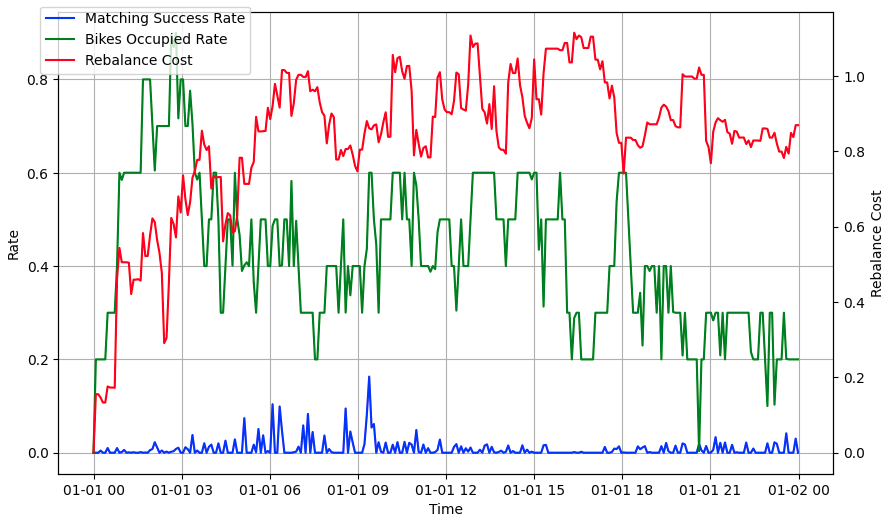
\includegraphics[scale=0.25]
          {figures/dispatchedResultFor1Day.png}
          \vspace{-5mm}
          \caption{自転車の割り当て成功率とステータスの変化}
          \label{fig:resultFig}
          \vspace{-5mm}  % 図の後のスペースを減らす
        \end{figure}

        \par 同様に,ベースラインとして構築した3つのモデルに対してもトリップデータを取り込み,自転車の割り当て処理を行い,比較評価指標としての再配置コストを比べた結果が図\ref{fig:モデル別再配置コストの時間経過比較}の通りである.
        \par NYCに配置する自転車数をスケールアップさせた場合についての検証も行うため,自転車の初期配置数50台にした場合の結果は図\ref{fig:50台の時の再配置コストの時間経過比較}にて示す通りである.さらに,初期配置する自転車を100台にスケールアップし,同様にシミュレーションを行ってみるも,50台の場合と比べて大きな変化は見られなかった.

        \begin{figure}[b]
          \centering
          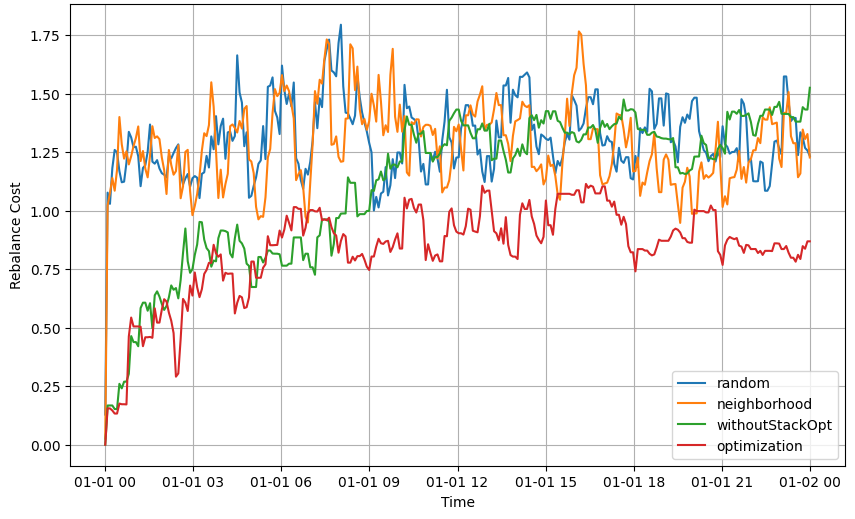
\includegraphics[scale=0.36]
          {figures/CompareRebalanceCost.png}
          \caption{モデル別再配置コストの時間経過比較}
          \label{fig:モデル別再配置コストの時間経過比較}
        \end{figure}

        \begin{figure}[b!]
          \centering
          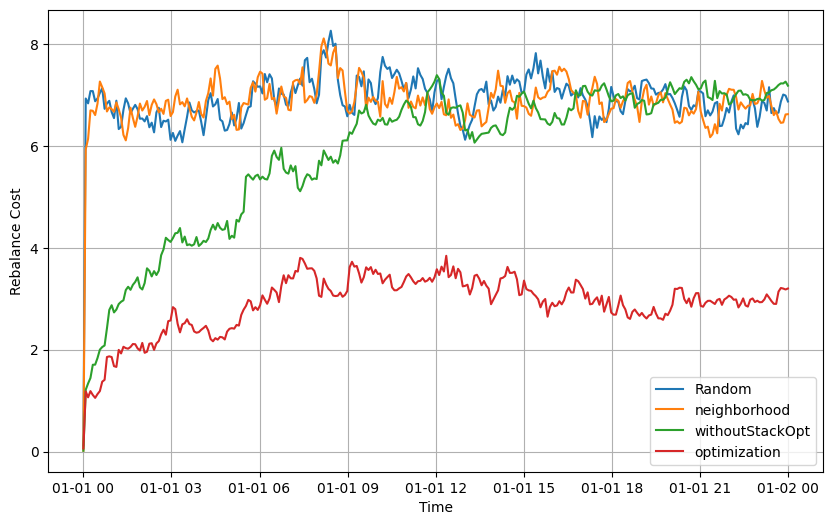
\includegraphics[scale=0.36]
          {figures/CompareRebalanceCost-50.png}
          \caption{50台の時の再配置コストの時間経過比較}
          \label{fig:50台の時の再配置コストの時間経過比較}
        \end{figure}

    \vspace{-5mm}

    % 第5章
    \section{考察}
        \label{sec:考察}
        \vspace{-3mm}
        \par 図\ref{fig:resultFig}の結果について,NYCに対してランダムに配置している自転車の数が10台である点が,タクシーのリクエスト数に対して圧倒的に不足しており,割り当て成功率が極端に低く推移している原因と考えられる.ただ,図\ref{fig:モデル別再配置コストの時間経過比較}で示した,同条件で割り当て処理を行ったモデル別の結果を参照すると,本研究で提案及び実装したバッチ最適化割り当てモデルが,再配置コストの観点で最も有意な結果であると捉えることができる.
        \par 図\ref{fig:50台の時の再配置コストの時間経過比較}の結果について,初期配置する自転車を50台にスケールアップした場合でも,やはり7万以上のユーザーリクエストに対しては非常に不足している状態であるため,割り当て成功率の上昇は期待できなかったが,それでも別モデルと比較した場合,自転車数をスケールアップした場合の方が,再配置コストにより有意性が増していることから,スケールメリットを持つ割り当てモデルであることが期待される.
        \par また,本研究では都合上,タクシーのトリップデータを扱ったが,自転車による移動を考慮すると,実験結果よりもより小さい値で再配置コストが推移する可能性も十分考えられる.

    \vspace{-5mm}

    % 第6章
    \section{結言}
        \label{sec:結言}
        \vspace{-3mm}
        \par 本研究では,CtoCシェアサイクルのための自転車割り当てモデルを構築し,実際のNYCのタクシーデータに基づきリクエストに対して自転車をユーザに割り当てることができた.今後の課題として,よりスケールアップさせたシミュレーションデータによる検証や,ユーザ体験とシステム効率性のトレードオフの最適解を探り,CtoCシェアサイクルの社会実装に向けたアプリケーションの拡充を目指す.

    \vspace{-5mm}

    % 参考文献
    \bibliographystyle{junsrt}
    \bibliography{references}

\end{document}
